% !TEX encoding = UTF-8 Unicode
\documentclass[a4paper]{article}

\usepackage[utf8]{inputenc}
\usepackage{erk}
\usepackage{amsmath}
\usepackage{times}
\usepackage{graphicx}
\usepackage{hyperref}
\usepackage[top=22.5mm, bottom=22.5mm, left=22.5mm, right=22.5mm]{geometry}

\usepackage[slovene,english]{babel}

% local definitions
\def\footnotemark{}%  to avoid footnote on cover page

\begin{document}
%make title
\title{The impact of input signal deformation on atan2 angle calculation error}
\author{Mitja Alič}
\affiliation{Faculty of Electrical Enginering, University of Ljubljana, Tržaška cesta 25, 1000 Ljubljana}
\email{E-mail: mitja1357@gmail.com}
\maketitle

\begin{abstract}{}
In position sensing encoders and resolvers are used, whose output is a pair of quadrature sine and cosine signals. Angle calculation can be done with atan2 function. Due to improper installation of sensor, sine and cosine signal can be deformed. In that case calculated angle includes error. Error was analyzed for non-equal amplitudes, non-orthogonality, DC offset and common mode signal. Error was analyzed in frequency specter, that yielded a function of error based on input signal deformation. Error is presented in Fourier series form.
\end{abstract}

\selectlanguage{English}

\section{Introduction}
These days the need for high quality motor regulation is present in numerous applications and has as a result become unavoidable. For a consistent and reliable measurement of rotation, position sensors are used \cite{uporaba_senzorjev}, such as encoders and resolvers \cite{inkrementalni}\cite{resolver}\cite{enkoder}. Because the output of such sensors is a pair of quadrature sine and cosine signals, angle must first be calculated. The easiest way of doing so is by directly calculating atan2, which returns a value between $[-\pi, \pi]$.

Because position sensors are not ideal, obtained sine and cosine signal can be deformed, phase shifted and DC offset. All of these imperfections cause the calculated angle to also include error.

Literature  \cite{orbis}, \cite{RLS1}, \cite{RLS2} and \cite{RLS3} analyses the impact of such imperfection for lower harmonics only and states that error of imperfections scale linearly. During our research we found, that the error specter also contains higher harmonics. The paper examines error waveform dependent on input signal mismatch with Fourier analysis. 

\section{Methodology and results}
Output from a position sensor can be represented with
\begin{eqnarray}
\label{equ:def_sin}
&Sin = B_{0} + B_1 \sin(\theta + \varphi_{s}) + CMM\\
\label{equ:def_cos}
&Cos = A_{0} + A_1 \cos(\theta + \varphi_{c}) + CMM
\end{eqnarray}

Where $B_0$ and $A_0$ represent DC offset, $B_1$ and $A_1$ signal amplitude, $\varphi_s$ and $\varphi_c$  phase shift and $\theta$ reference angle. Signals (\ref{equ:def_sin}) and (\ref{equ:def_cos}) can also have a common superimposed AC signal  represented as CMM (\ref{equ:CMM}). CMM can be of cosine or sine form with $\Delta_c$ and $\Delta_s$ as amplitude.

\begin{equation}
\label{equ:CMM}
CMM = \Delta_c \cos(\theta)+\Delta_s \sin(\theta)
\end{equation}
By calculating atan2 for eq. (\ref{equ:def_sin}) and (\ref{equ:def_cos})
\begin{equation}
\label{equ:def_kot}
\varphi = \mathrm{atan2}(Sin,Cos)
\end{equation}
and then subtracting it with an unaltered signal
\begin{equation}
\label{equ:def_err}
\varepsilon =\varphi - \mathrm{atan2}(\sin(\theta),\cos(\theta))
\end{equation}
we get error based on deformation. Because  AC signal analysis is simpler in frequency domain, error was converted with Fast Fourier Transform(FFT). By varying each parameter individually we examined the impact of the parameter in question on specter of error. Output of atan2 was examined by sending each parameter in eq. (\ref{equ:def_sin}) and (\ref{equ:def_cos}) to infinity or worst case with phase shift.
In this case amplitude and phase of each harmonic approaches to a limit value.

The course of the amplitude and phase in dependence on the changing parameter was approximated by a function, that best suited numerical waveform obtained from the error spectrum. The set of functions decreases by checking the limit value to which each amplitude and phase approach. We were looking for the best approximation with polynomials, rational functions, exponential, trigonometric and cyclometric functions. The best approximation was sought using the minimum squares method.

\subsection{Defining of error at different amplitudes}
In the first case was observed the impact of different amplitudes on error. The output of the atan2 function is determined by the eq. (\ref{equ:def_sin}) and (\ref{equ:def_cos}) quotient. Since only the ratio of the amplitudes needs to be preserved, we multiplied both signals by $\frac{1}{A_1}$. By changing only the amplitudes in (\ref{equ:def_sin}) and (\ref{equ:def_cos}), input signals are:
	\begin{eqnarray}
	\label{equ:def_sin_ama}
	&Sin = k \sin(\theta),\\
	\label{equ:def_cos_amp}
	&Cos =\cos(\theta),
	\end{eqnarray}
where $k$ represents $\frac{B_1}{A_1}$.

By varying the parameter $k$ from 0 to infinity, it was found that, the error specter consists of even harmonics only. It was also observed that phase shift didn't change. When $k$ approaches infinity, the amplitude of harmonics approaches $\frac{180}{\pi}\frac{2}{n}$, where n represents n-th harmonic. Eq. (\ref{equ:lim_amp_vrsta}) which contains even harmonics only.
\begin{equation}
\label{equ:lim_amp_vrsta}
\varepsilon(k \rightarrow \infty) = \frac{180}{\pi}\sum_{n=1}^{\infty}\frac{1}{n} \sin 2 n \theta
\end{equation}
Because second harmonic is the largest, we approximated it first (Figure \ref{fig:amp}).
\begin{figure}[!htb]
	\begin{center}
		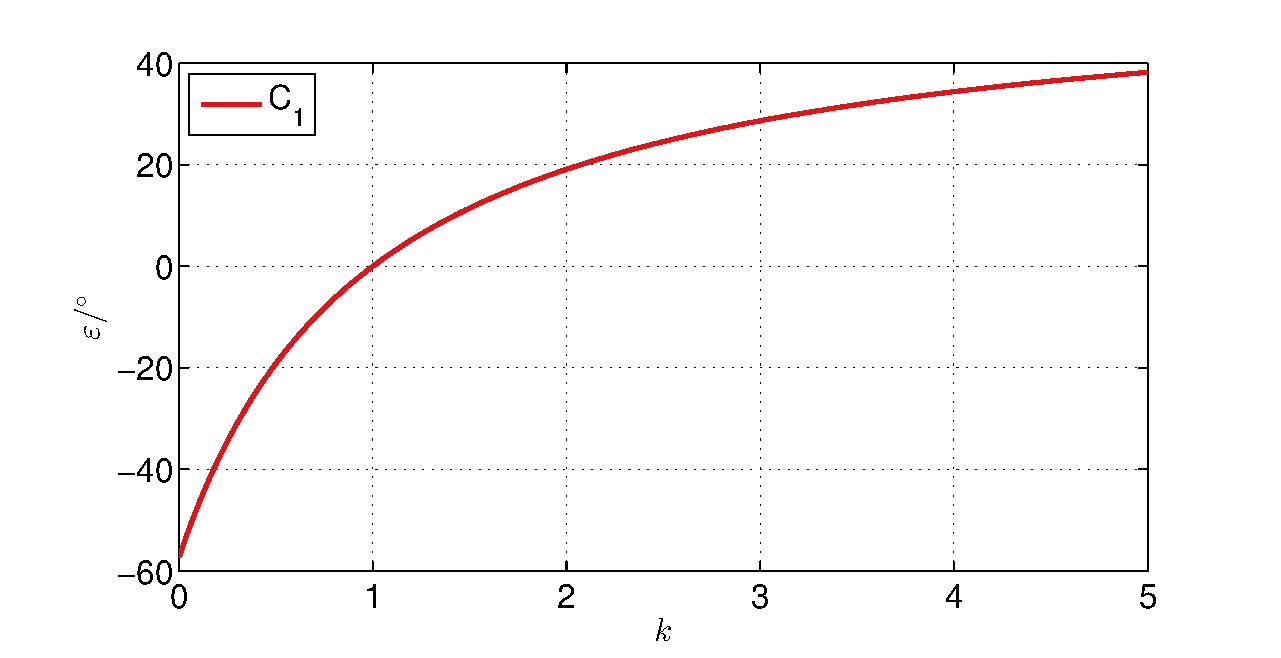
\includegraphics[width=\linewidth]{./Slike/amp.eps}
		\caption{Waveform of the second harmonic depending on $k$} \label{fig:amp}
	\end{center}
\end{figure}

Best approximation was rational function  (\ref{equ:drugi_har}), with summed squared error (SSE) $1.18 \cdot 10^{-10}$ degrees.
\begin{eqnarray}
\label{equ:drugi_har}
C_2(k)=\frac{180}{\pi}\cdot\frac{k-1}{k+1}
\end{eqnarray}

It was assumed, that higher order harmonics were correlated with base harmonic. Function, that describes error  depending on $k$ is presented in Fourier series form (\ref{equ:amp_err}).
\begin{equation}
\label{equ:amp_err}
\varepsilon(k) =\frac{180}{\pi}\sum_{n=1}^{\infty}\frac{1}{n}(\frac{k-1}{k+1})^n \sin 2 n \theta
\end{equation}
By replacing $k$ with ratio of amplitudes $\frac{B_1}{A_1}$, we get final equation
\begin{equation}
\label{equ:amp_err2}
\varepsilon(A_1, B_1) =\frac{180}{\pi}\sum_{n=1}^{\infty}\frac{1}{n}(\frac{B_1-A_1}{B_1+A_1})^n \sin 2 n \theta,
\end{equation}
which is valid for positive ratio of amplitudes only.
 $$\frac{B_1}{A_1} \geq 0.$$

\subsection{Defining of error at non-orthogonality}
In second case, it was examined the impact of phase deformation. Input signals are represented as:
\begin{eqnarray}
\label{equ:def_sin_fis}
&Sin = \sin(\theta + \varphi_{s})\\
\label{equ:def_cos_fis}
&Cos =\cos(\theta+\varphi_{c})
\end{eqnarray}
Error was analyzed for $\varphi_s$ and $\varphi_c$ individually, in the end equations were combined.

Worst case of error is, when $\varphi_s$ approaches $90^\circ$ and can be presented as Fourier series (\ref{equ:lim_fis_vrsta}). Error consists of DC component and even harmonics only.
\begin{equation}
\label{equ:lim_fis_vrsta}
\varepsilon(\varphi_{s} \rightarrow 90^\circ) = 45^\circ - \frac{180}{\pi}\sum_{n=1}^{\infty}\frac{1}{n} \sin (2n \theta)
\end{equation}
Correlation between amplitudes and $\varphi_{s}$ yields tangent function (Figure \ref{fig:fis}). DC component and phase of error were being changed linearly. Tangent function approximate second harmonic with SSE of $1.18 \cdot 10^{-10}$ degrees.
\begin{figure}[!htb]
	\begin{center}
		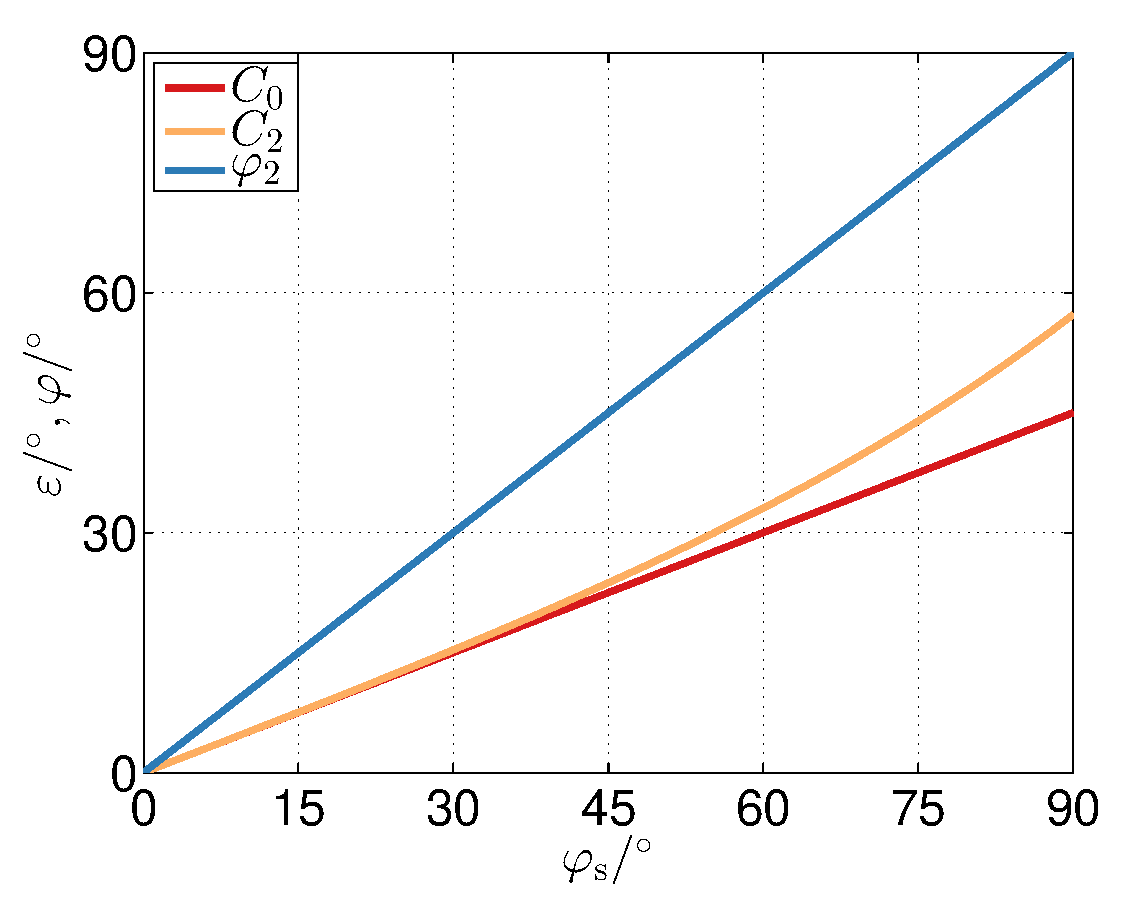
\includegraphics[width=\linewidth]{./Slike/fis.eps}
		\caption{Waveforms of DC component $C_0$, amplitude of second harmonic  $C_2$ and phase of second harmonic $\varphi_2$ compared to ideal cosine signal, due to phase shift $\varphi_{s}$} \label{fig:fis}
	\end{center}
\end{figure}

Same procedure can be applied for parameter $\varphi_c$ as well.
Because error from (\ref{equ:def_sin_fis}) and (\ref{equ:def_cos_fis}) is independent, their contribution can be combined into (\ref{equ:fis_err}).
\begin{multline}
\label{equ:fis_err}
\varepsilon(\varphi_{s},\varphi_{c}) = \frac{\varphi_{s}+\varphi_{c}}{2}+\\ \frac{180}{\pi}\sum_{n=1}^{\infty}\frac{1}{n} (\mathrm{tan}\frac{\varphi_{s}-\varphi_{c}}{2})^n \sin (2n \theta+n(90^\circ +\varphi_{s}+\varphi_{c}))
\end{multline}
Expression (\ref{equ:fis_err}) is valid only for range:
$$ \varphi_{s}-\varphi_{c} \in [ -90^\circ , 90^\circ ] $$

\subsection{Defining of error for DC component in one input signal only}
\label{DCoff}
By varying DC component in (\ref{equ:def_sin}) and (\ref{equ:def_cos}) equations are:
\begin{eqnarray}
&Sin = sin(\theta)+ B_0\\
&Cos = cos(\theta) + A_0.
\end{eqnarray}
When parameter $A_0$ approaches infinity, error is described by eq. (\ref{equ:off_lim_vrsta}).
\begin{equation}
\label{equ:off_lim_vrsta}
\varepsilon (A_0 \rightarrow \infty) = \frac{180}{\pi}\sum_{n=1}^{\infty}\frac{2}{n} \sin (n \theta + n 180^\circ).
\end{equation}
Error does not contain DC component and the highest harmonic is the first.
\begin{figure}[!htb]
	\begin{center}
		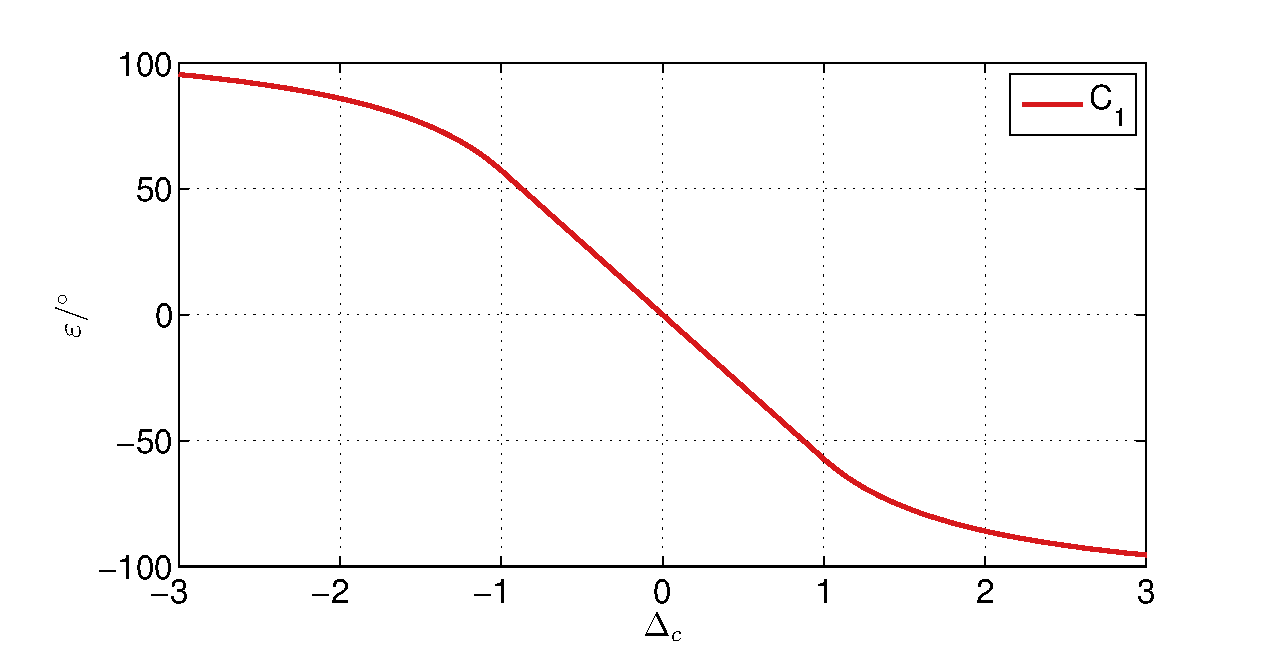
\includegraphics[width=\linewidth]{./Slike/off.eps}
		\caption{Amplitude of first harmonic depending on  $\frac{A_0}{A_1}$} \label{fig:off}
	\end{center}
\end{figure}
The waveform from figure \ref{fig:off}, was split into 3 parts based on ratio between offset and amplitude. Expression which best approximate waveform of first harmonic of error with SSE of $1.21 \cdot 10^{-7}$ degrees is in exponential and linear form (\ref{equ:offc_err}):
\begin{multline}
\label{equ:offc_err}
\varepsilon(A_0, A_1)=\\
\begin{cases}
\frac{180}{\pi}\sum_{n=1}^{\infty} \frac{1}{n}(2-|\frac{A_0}{A_1}|^{-n}) \sin (n \theta ), & \frac{A_0}{A_1}\leq -1 \\
\frac{180}{\pi}\sum_{n=1}^{\infty}(-1)^n\frac{1}{n}(\frac{A_0}{A_1})^n \sin (n \theta ), & |\frac{A_0}{A_1}|\leq 1 \\
\frac{180}{\pi}\sum_{n=1}^{\infty}(-1)^n\frac{1}{n}(2-(\frac{A_0}{A_1})^{-n}) \sin (n \theta ), & \frac{A_0}{A_1}\geq 1
\end{cases}
\end{multline}
Same procedure can be applied for parameter $B_0$ as well. Result is eq. (\ref{equ:offs_err}).
\begin{multline}
\label{equ:offs_err}
\varepsilon(B_0, B_1)=\\
\begin{cases}
\frac{180}{\pi}\sum_{n=1}^{\infty}\frac{1}{n}(2-|\frac{B_0}{B_1}|^{-n}) \sin (n \theta -  90^\circ n), & \frac{B_0}{B_1}\leq -1 \\
\frac{180}{\pi}\sum_{n=1}^{\infty}\frac{1}{n}(\frac{B_0}{B_1})^n \sin (n \theta + 90^\circ n), & |\frac{B_0}{B_1}|\leq 1 \\
\frac{180}{\pi}\sum_{n=1}^{\infty}\frac{1}{n}(2-(\frac{B_0}{B_1})^{-n}) \sin (n \theta^\circ + 90 n), & \frac{B_0}{B_1}\geq 1
\end{cases}
\end{multline}

\subsection{Defining of error for common DC component in both input signals}
Input signals can also contain common DC component. 
This happens when resolvers stator coils are improperly install. Same analysis as in subsection \ref{DCoff} can be applied in this case as well. Result is presented in eq. (\ref{equ:offsc_err}).
\begin{multline}
\label{equ:offsc_err}
\varepsilon(A_0,B_0=A_0, A_1)=\\
\begin{cases}
\frac{180}{\pi}\sum_{n=1}^{\infty}\frac{1}{n}(2-|\sqrt{2}\frac{A_0}{A_1}|^{-n}) \sin (n \theta - 45^\circ n), & \frac{A_0}{A_1}\leq -\frac{\sqrt{2}}{2} \\
\frac{180}{\pi}\sum_{n=1}^{\infty}\frac{1}{n}(\sqrt{2}\frac{A_0}{A_1})^n \sin (n \theta + 135^\circ n), & |\frac{A_0}{A_1}|\leq \frac{\sqrt{2}}{2} \\
\frac{180}{\pi}\sum_{n=1}^{\infty}\frac{1}{n}(2-(\sqrt{2}\frac{A_0}{A_1})^{-n}) \sin (n \theta +135^\circ n), & \frac{A_0}{A_1}\geq \frac{\sqrt{2}}{2}
\end{cases}
\end{multline}

\subsection{Impact of CMM signal on error}
CMM signal is the result of  improper resolvers rotor part installation.

By limiting error of $\Delta_c$ to infinity.
Because CMM effects amplitude mismatch and non-orthogonality of input signals, error was expected to contain DC component and even harmonics only.
Error when $\Delta_c$ approaches infinity, is presented in (\ref{equ:lim_dc_vrsta}).
\begin{equation}
\label{equ:lim_dc_vrsta}
\varepsilon(\Delta_c \rightarrow \infty) = 45^\circ -\frac{180}{\pi}\sum_{n=1}^{\infty}\frac{1}{n} \sin( 2 n \theta).
\end{equation}
Because general approximation was not found, error specter was split into sine and cosine part (\ref{sincospart}).
\begin{equation}
\label{sincospart}
C_{ns}(\Delta_c) \cdot\sin(n\theta)+C_{nc}(\Delta_c) \cdot\cos(n\theta)
\end{equation}
Figure \ref{fig:dc} presents split second harmonic and DC component.
\begin{figure}[!htb]
	\begin{center}
		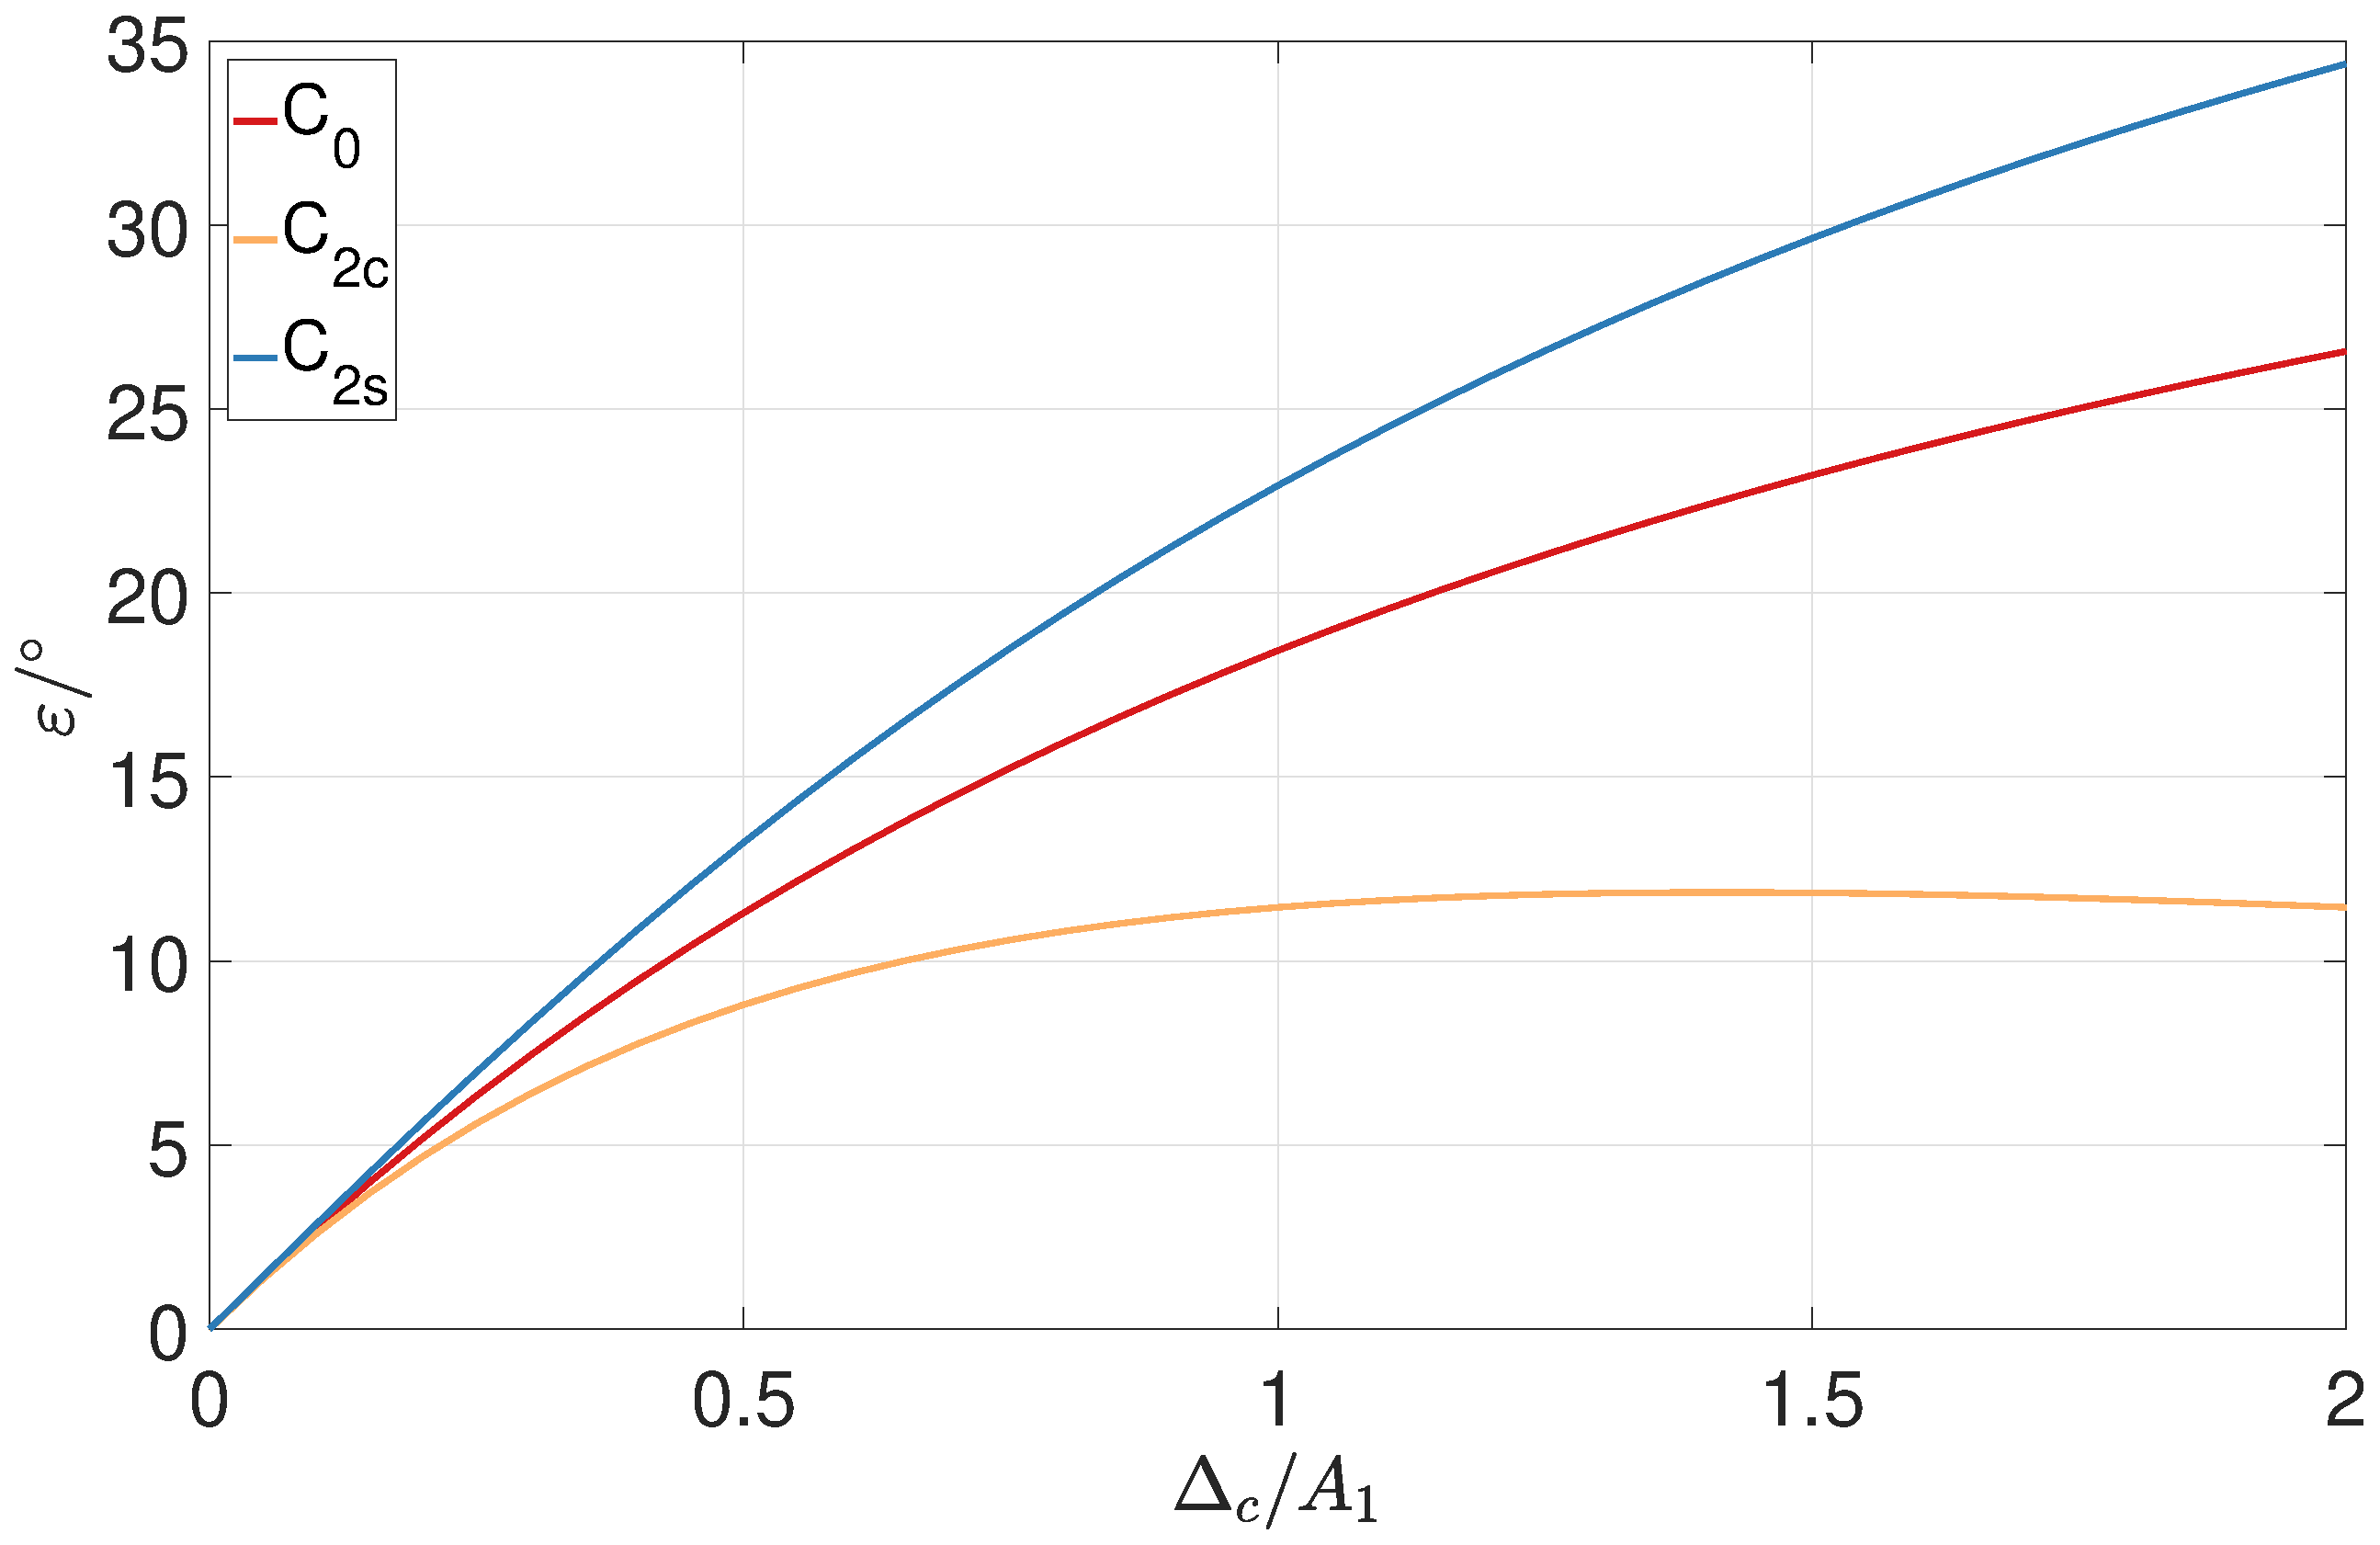
\includegraphics[width=\linewidth]{./Slike/dc.eps}
		\caption{Waveform of DC component and split second harmonic depending on $\frac{\Delta_{c}}{A_1}$} \label{fig:dc}
	\end{center}
\end{figure}

DC component was approximated with SSE of $1.94 \cdot 10^{-22}$ degrees with atan function. Waveform of $C_{2s}$ and $C_{2c}$ were approximated with SSE to less then $1.15 \cdot 10^{-9}$ degrees.
Final function, that described error depending on $\Delta_c$ is presented in Fourier series form (\ref{equ:dc_err}).
\begin{multline}
\label{equ:dc_err}
\qquad\varepsilon(A_1, \Delta_c) = \mathrm{atan}\frac{\Delta_c}{\Delta_c+2 A_1}+\\
\qquad+\frac{180}{\pi} \sum_{n=1}^{\infty}\frac{1}{n} (\frac{\Delta_c}{\sqrt{\Delta_c^2+2 A_1 \Delta_c+2 A_1}})^n\\ \sin (2n \theta+n (90^\circ+ \mathrm{ atan}(\frac{\Delta_c+A_1}{A_1})))
\end{multline}

Same procedure can be applied for parameter $\Delta_s$ as well. Result is eq.(\ref{equ:ds_err})
\begin{multline}
\label{equ:ds_err}
\varepsilon(A_1, \Delta_s) = -\mathrm{atan}\frac{\Delta_s}{\Delta_s+2 A_1}+\\+\frac{180}{\pi} \sum_{n=1}^{\infty}\frac{1}{n} (\frac{\Delta_s}{\sqrt{\Delta_s^2+2 A_1 \Delta_s+2A_1}})^n\\ \sin (2n \theta+n (90^\circ- \mathrm{ atan}(\frac{\Delta_s+A_1}{A_1})))
\end{multline}

Eq. (\ref{equ:dc_err}) and (\ref{equ:ds_err}) are valid for only: 
\begin{equation*}
\Delta_s, \Delta_c > -A_1
\end{equation*}

\section{Comment on results}
After defining error due to deformation parameter in input signal, a fault of approximation (\ref{equ:def_err}) was made. Approximated functions were defined with infinite series, during analysis of fault were used first 15 components only. In example input signals have amplitudes $A_1 = 1$ and $B_1 = 1.1$. Difference between error calculated with (\ref{equ:amp_err2}) and error from (\ref{equ:def_err})  is presented in figure \ref{fig:razlika}. Fault of approximation is in the vicinity of a numeric error. Comparing errors in frequency specter, showed minimum deviations between harmonics of same frequency.

It is necessary to mention that despite the derivation, the presented types of errors of individual deformations still depends on each other.
\begin{figure}[!htb]
	\begin{center}
		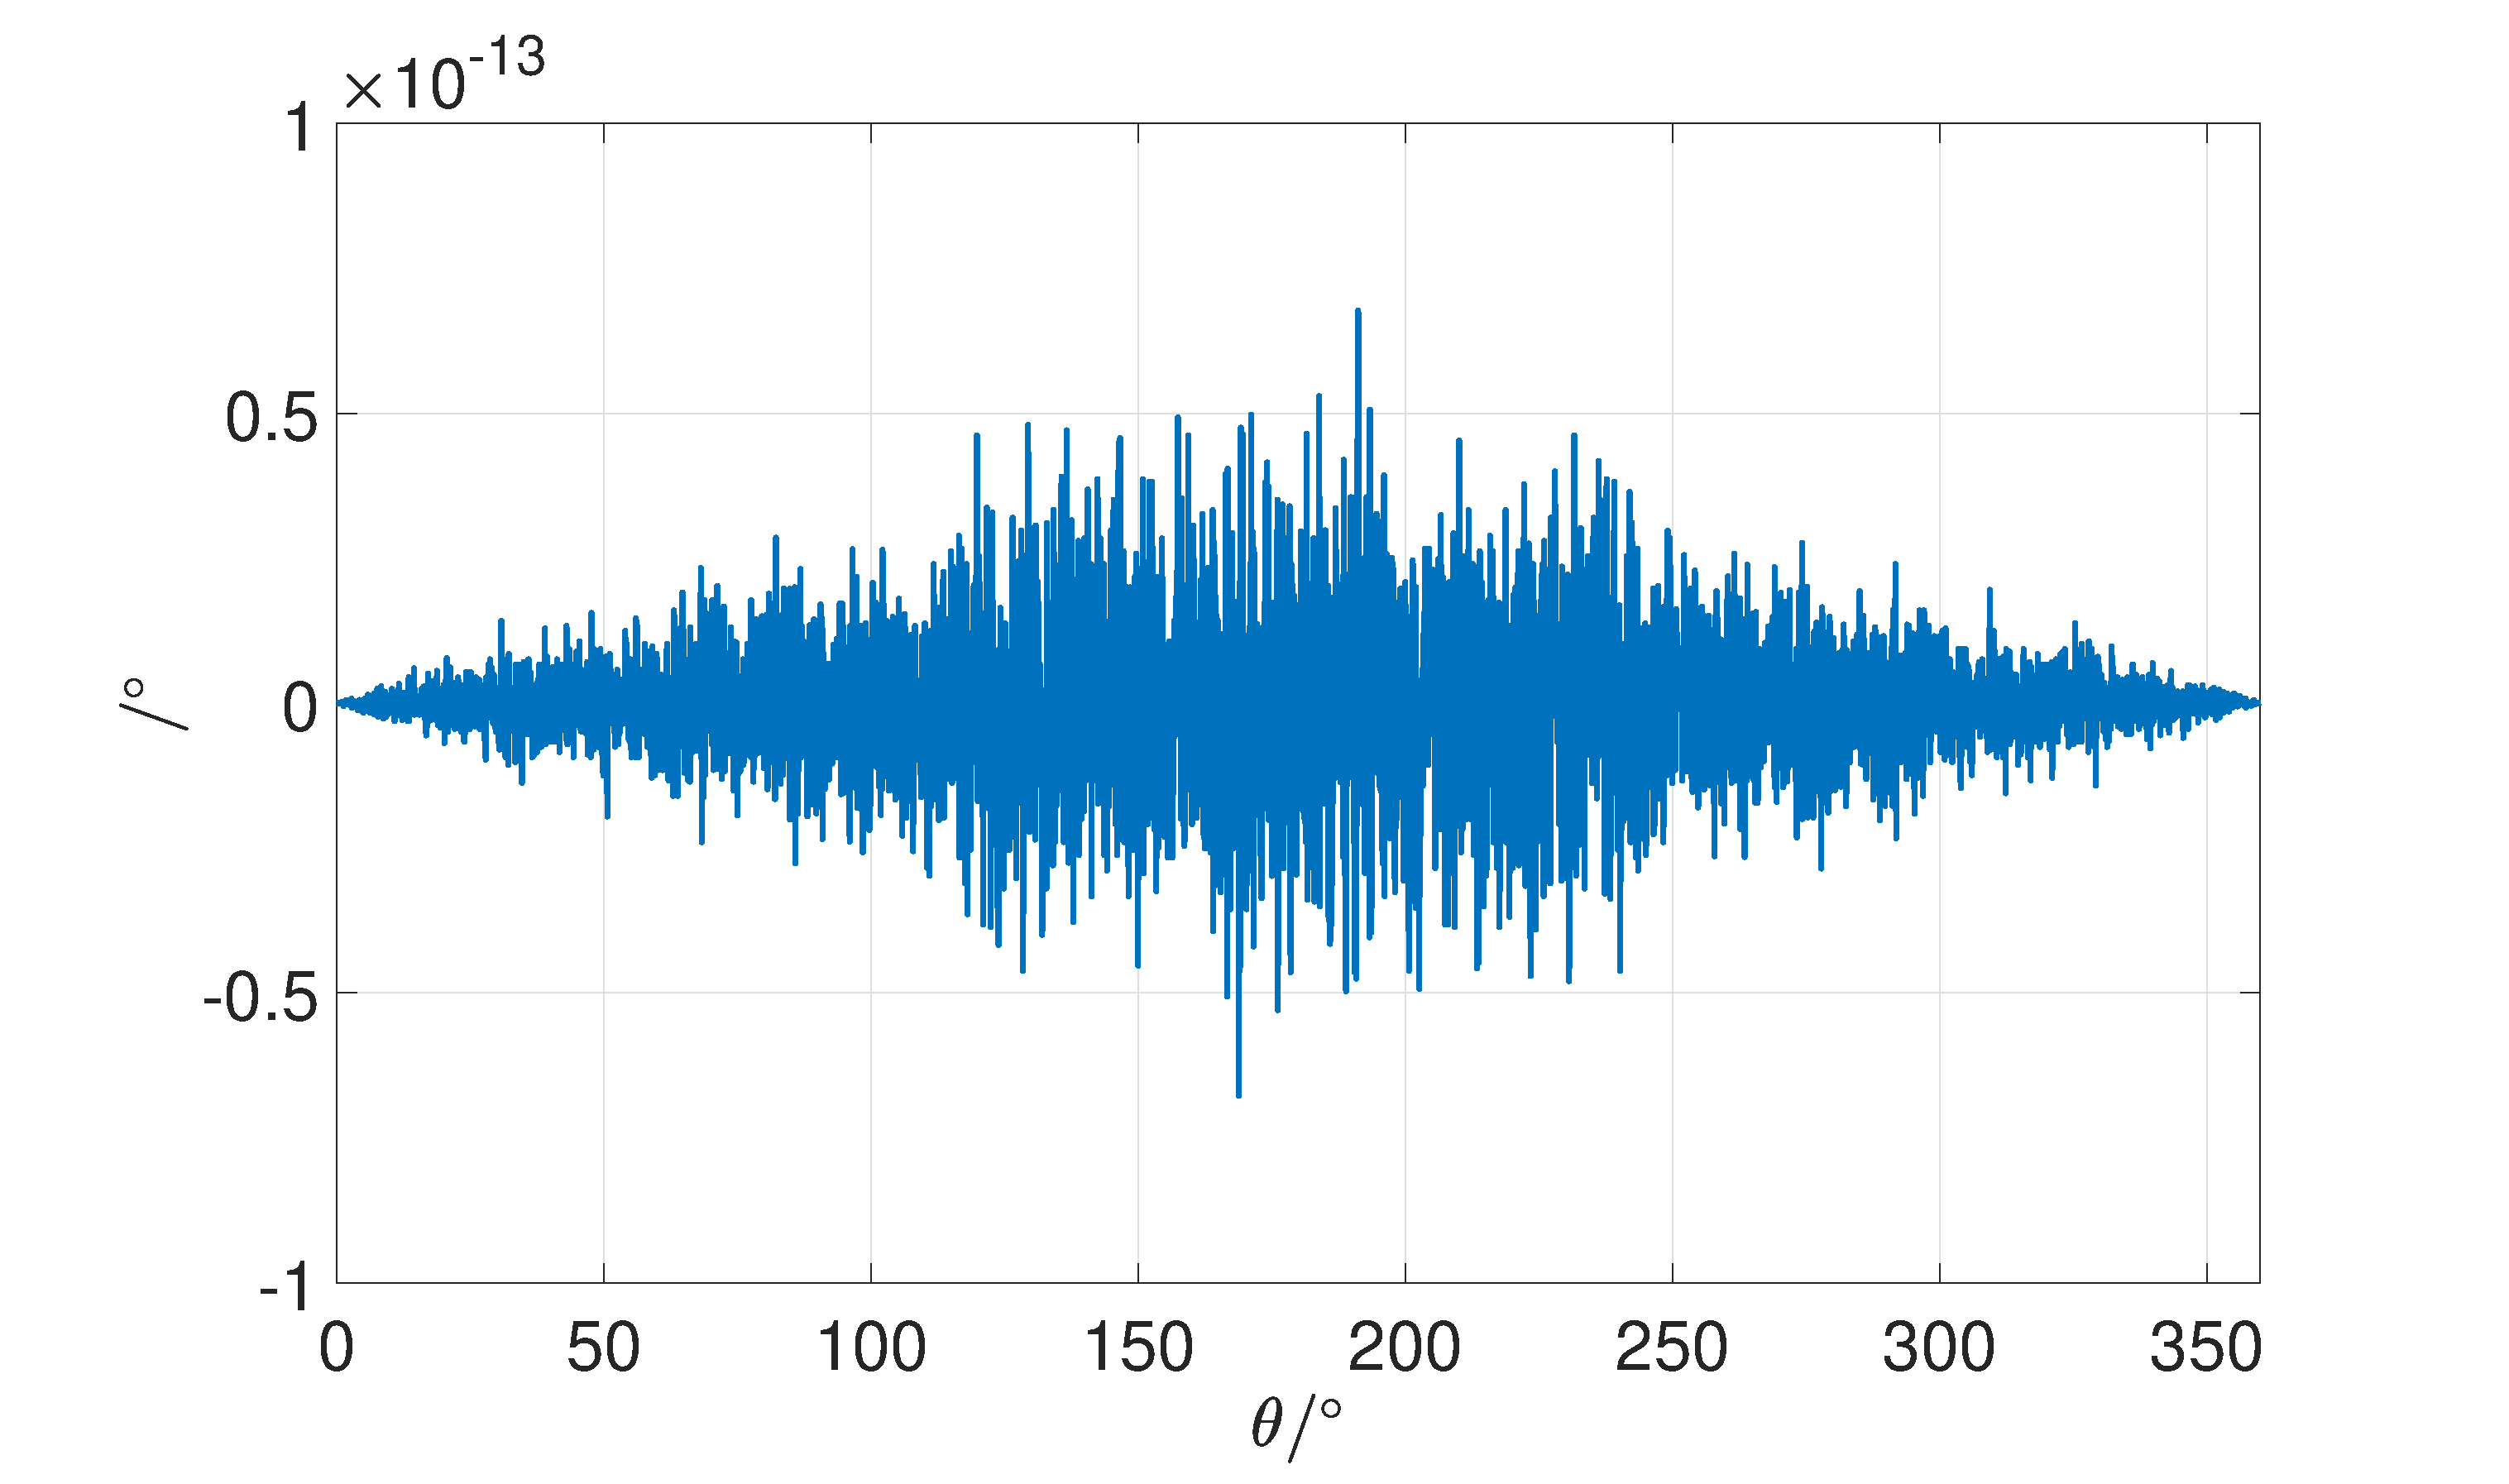
\includegraphics[width=\linewidth]{./Slike/razlika_amp.eps}
		\caption{Difference between predicted (\ref{equ:amp_err2}) and actual error} \label{fig:razlika}
	\end{center}
\end{figure}

\section{Conclusion}
With methods described in this paper, improper installation of encoders and resolvers can be uncovered from analyzing error only.
Content of higher harmonics in error become non-negligible at major mismatches. This paper presents impact of signal mismatch, non-orthogonality, DC offset and common mode signal to output error of atan2 function.

Input signals can include higher harmonics distortion, which is not described in this paper. The impact of distortion of the input signals in the atan2 function to the output error offers many challenges for further work. 
\small
%\section*{Acknowledgment}
%This paper could not be possible without the help of my friend and colleague Draš Kunšič. I am deeply grateful for his generous help and encouragement.


\begin{thebibliography}{1}
\bibitem{uporaba_senzorjev} Gachter J., Hirz M.,Seebacher R., "Impact of Rotor Position Sensor Errors on Speed
Controlled Permanent Magnetized Synchronous
Machines", IEEE 12th International Conference on Power Electronics and Drive Systems (PEDS), pp.822-830, 12-15 Dec. 2017

\bibitem{inkrementalni} Brugnano F., Concari C., Imamovic E., Savi F., Toscani  A., Zanichelli R., "A simple and accurate algorithm for speed measurement in electric drives using incremental encoder",
IECON 2017 - 43rd Annual Conference of the IEEE Industrial Electronics Society, pp. 8551-8556, 29 Oct.-1 Nov. 2017

\bibitem{resolver} Reddy B.P., Murali A., Shaga G., "Low Cost Planar Coil Structure for Inductive Sensors to Measure Absolute Angular
Position", 2017 2nd International Conference on Frontiers of Sensors Technologies (ICFST), pp.14-18, 14-16 April 2017

\bibitem{enkoder} Zhang Z., Ni F., Liu H., Jin M., "Theory analysis of a new absolute position sensor based on electromagnetism", International Conference on Automatic Control and Artificial Intelligence, pp.2204-208, 3-5 Mar. 2012

\bibitem{orbis} Lara J., Chandra A., "Position Error Compensation in Quadrature
Analog Magnetic Encoders through an Iterative
Optimization Algorithm",  IECON 2014 - 40th Annual Conference of the IEEE Industrial Electronics Society, pp.3043-3048, 29 Oct.-1 Nov. 2014 
	
\bibitem{RLS1} Qi Lin, T. Li, Z. Zhou, "Error Analysis and Compensation
of the Orthogonal Magnetic Encoder", Proceedings of IEEE ICMCC
Conference, pp.11-14, 21-23 Oct. 2011

\bibitem{RLS2} Hanselman D.C., "Resolver Signal Requirements for High Accuracy
Resolver-to-Digital Conversion", IEEE Transactions on Industrial
Electronics, vol.37, no.6, pp.556-561, Dec. 1990 

\bibitem{RLS3} Demierre M., “Improvements of CMOS Hall Microsystems and
Application for Absolute Angular Position Measurements”, PhD. thesis,
pp. 152-161, Federal Polytechnic School of Lausanne, Switzerland, 2003
%\bibitem{mat1} Dolinar G. "Matematika 1", Fakulteta za elektrotehniko, Založba FE in FRI, 2010
%\bibitem{atan} https://www.mathworks.com/help/matlab/ref/atan2.html, dostop junij 2018
\end{thebibliography}
\end{document}
